\documentclass{article}
\usepackage{setspace}
\usepackage{amsmath}
\usepackage{amssymb}
\usepackage{amsthm}
\usepackage{graphicx} 
\usepackage{float} 
\usepackage{fancyhdr}                                
\usepackage{lastpage}        
\usepackage{textcomp}                               
\usepackage{layout}   
\usepackage{subfigure} 
\pagestyle{fancy}  
\lhead{ZHANG HUAKANG}
\chead{Assignment 1} 
\rhead{DB92760} 
\renewcommand{\baselinestretch}{1.05}
\title{Assignment 1 of CISC 1006}
\author{ZHANG HUAKANG \\ DB92760 \\ \\ Computer Science, \\Faculty of Science and Technology}
\begin{document}
    \maketitle
    \section{}
            \paragraph{
                \begin{tabular}{c|c|c}
                    \hline
                    1 &H &H \\
                    &H & T\\
                    & T&H \\
                     & T&T \\
                    \hline
                    2 & H& \\
                     & T& \\
                    \hline
                    3&H &H \\
                    & H&T \\
                    & T&H \\
                    & T&T \\
                    \hline
                    4&H & \\
                    &T & \\
                    \hline
                    5&H &H \\
                    & H&T \\
                    & T&H \\
                    & T&T \\
                    \hline
                    6&H & \\
                    &T & \\
                    \hline
                \end{tabular}
            }
        \subsection{}
            \paragraph{
                $$A=\{1HH,1HT,1TH,1TT,2H,2T\}$$
            }
        \subsection{}
            \paragraph{
                \begin{equation*}
                    \begin{split}
                        B=\{& 1HH,1HT,1TH,1TT,\\
                            &3HH,3HT,3TH,3TT,\\
                            &5HH,5HT,5TH,5TT\}\\
                    \end{split}
                \end{equation*}
            }
        \subsection{}
            \paragraph{
                \begin{equation*}
                    \begin{split}
                        A'=\{& 4H,4T,6T,6H,\\
                            &3HH,3HT,3TH,3TT,\\
                            &5HH,5HT,5TH,5TT\}\\
                    \end{split}
                \end{equation*}
            }
        \subsection{}
            \paragraph{
                \begin{equation*}
                    \begin{split}
                        A'\cap B =\{&3HH,3HT,3TH,3TT,\\
                            &5HH,5HT,5TH,5TT\}\\
                    \end{split}
                \end{equation*}
            }
        \subsection{}
            \paragraph{
                \begin{equation*}
                    \begin{split}
                        A'\cup B =\{&1HH,1HT,1TH,1TT,\\
                            &3HH,3HT,3TH,3TT,\\
                            &5HH,5HT,5TH,5TT\\
                            &4H,4T\\
                            &6H,6T\}\\
                    \end{split}
                \end{equation*}
            }
    \section{}
        \subsection{}
            \begin{figure}[H]
                \centering
                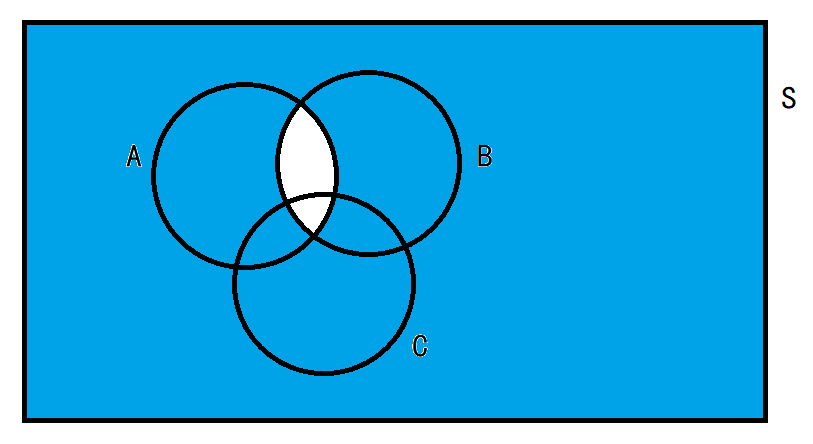
\includegraphics[width=0.9\textwidth]{img/Assignment1-01.png}
            \end{figure}
        \subsection{}
            \begin{figure}[H]
                \centering
                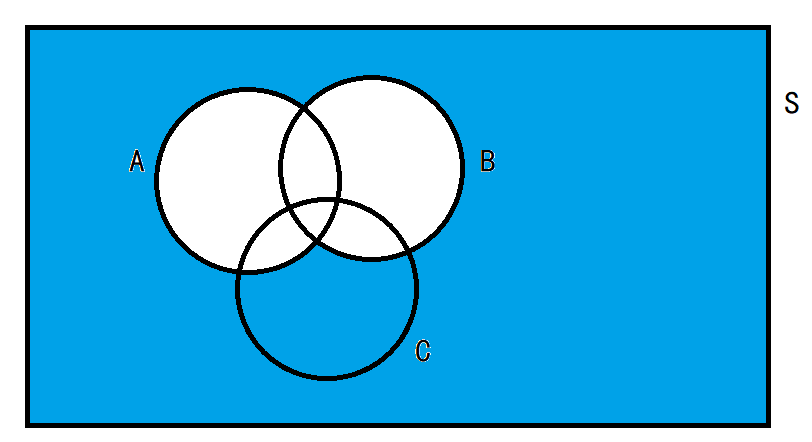
\includegraphics[width=0.9\textwidth]{img/Assignment1-02.png}
            \end{figure}
        \subsection{}
            \begin{figure}[H]
                \centering
                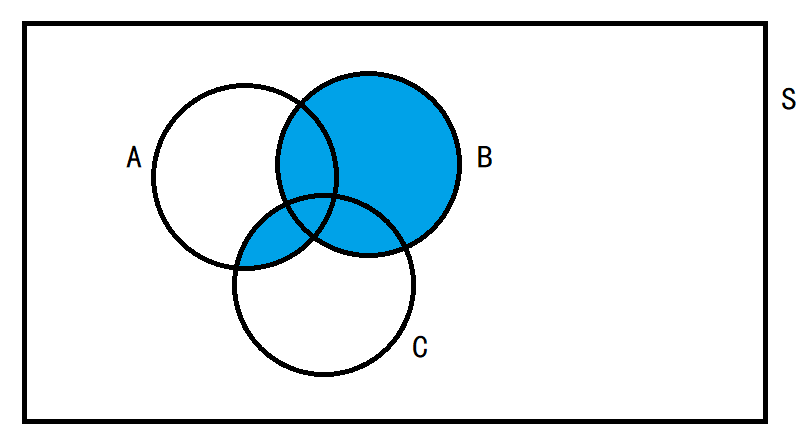
\includegraphics[width=0.9\textwidth]{img/Assignment1-03.png}
            \end{figure}
    
    \section{}
        \subsection{}
            \paragraph{
                $$P_6^6=720$$
            }
        \subsection{}
            \paragraph{
                $$P_4^4P_3^3=144$$
            }
        \subsection{}
            \paragraph{
                $$P_4^4P_5^2=480$$
            }
        \subsection{}
            \begin{itemize}
                \item $[1,4,4]$, $C_9^1C_8^4C_4^4=630$
                \item $[1,3,5]$, $C_9^1C_8^3C_5^5=504$
                \item $[2,2,5]$, $C_9^2C_7^2C_5^5=756$
                \item $[2,3,4]$, $C_9^2C_7^3C_4^4=1260$
                \item $[2,4,3]$, $C_9^2C_7^4C_3^3=1260$
            \end{itemize}
            $$Total= 4410$$
    \section{}
        \subsection{}
            \paragraph{
                $$C_5^4=5$$
            }
        \subsection{}
            \paragraph{
                $$C_5^1C_7^3=175$$
            }
        \subsection{}
            \paragraph{
                $$C_5^1C_7^3+C_5^2C_7^2+C_5^3C_7^1+C_5^4C_7^0=460$$
            }
        \subsection{}
            \paragraph{
                $$C_5^0C_7^4+C_5^1C_7^3+C_5^2C_7^2=420$$
            }
    \section{}
        \subsection{}
            \paragraph{
                $$0.19+0.38+0.29+0.15=1.01\neq 1$$
                We know that $$\mathbb{P}(S)=1$$ where $S$ is a sample space of any random experiment
            }
        \subsection{}
            \paragraph{
                $$0.4+0.52=0.92\neq 1$$
                We know that $$\mathbb{P}(S)=1$$ where $S$ is a sample space of any random experiment
            }
        \subsection{}
            \paragraph{
                The probability of a random event can equal to $-0.25$. We know that for any event $A$, the probability of $A$ should be nonnegative real number, i.e. $$\mathbb{P}(A)\geq 0$$
            }
        \subsection{}
            \paragraph{
                Heart is red. The probability of a card is balck heart is $0$
            }
    \section{}
        \paragraph{
            Let $A$ be the set of students who somke, $B$ be the set of students who drink alcholic beverages, and $C$ be the set of students who eat between meals. We know that the number of elements in ecah set is that 
            \begin{equation*}
                \begin{split}
                    |T|=&500\\
                    |A|=&210\\
                    |B|=&258\\
                    |C|=&216\\
                \end{split}
            \end{equation*}
            We also know that 
            \begin{equation*}
                \begin{split}
                    |A\cap B|=&122\\
                    |B\cap C|=&83\\
                    |A\cap C|=&97\\
                    |A\cap B\cap C|=&52
                \end{split}
            \end{equation*}
            % From this infomation, we can get that 
            \begin{equation*}
                \begin{split}
                    \emptyset=&(A\cap B'\cap C')\cup [(A\cap B)\cup (A\cap C)\cup(A\cap B\cap C)\\ 
                    A=&(A\cap B'\cap C')\cap [(A\cap B)\cup (A\cap C)\cup(A\cap B\cap C)\\    
                    |A\cap B'\cap C'|=&|A|-|(A\cap B)\cup (A\cap C)\cup(A\cap B\cap C)|\\
                    =&|A|-|A\cup B|-|A\cup C| +|A\cap B\cap C|\\
                    =&43\\     
                \end{split}
            \end{equation*}
            % It is same to get 
            \begin{equation*}
                \begin{split}
                    |B\cap A'\cap C'|=&105\\
                    |C\cap A' \cap B'|=&88,\\
                    (A\cap B \cap C)\cup(A\cap B \cap C')=&A\cap B\\
                    (A\cap B \cap C)\cap(A\cap B \cap C')=&\emptyset\\
                    |A\cap B \cap C|+|A\cap B \cap C'|=&|A\cap B|\\
                    |A\cap B \cap C'|=&70\\
                    |A\cap C \cap B'|=&45\\
                    |B\cap C \cap A'|=&31,\\
                \end{split}
            \end{equation*}
            and
            \begin{equation*}
                \begin{split}
                    (A\cup B\cup C)\cup (A'\cap B' \cap C')=&T\\
                    (A\cup B\cup C)\cap (A'\cap B' \cap C')=&\emptyset\\
                    |A\cup B\cup C|=&|A|+|B\cup A'|+|C\cup A'\cup B'|\\
                    =&433\\
                    |A'\cap B' \cap C'|=&|T|-|A\cup B\cup C|\\
                    =&67\\
                \end{split}
            \end{equation*}
        }
        \subsection{}
            \paragraph{
                The probability of a student somkes but does not drink alcholic beverages is 
                \begin{equation*}
                    \begin{split}
                        \mathbb{P}_1=&\frac{|A\cap B'|}{|T|}\\
                            =&\frac{|A\cap B'|+|C\cap B'|-|A\cap C\cap B'|}{|T|}\\
                            =&\frac{|A\cap B'|+|C\cap B'|-(|A\cap C|-|A\cap B \cap C|))}{|T|}\\
                            =&\frac{(|A|-|A\cap B|)+(|C|-|B\cap C|))-(|A\cap C|-|A\cap B \cap C|))}{|T|}\\
                            =&\frac{88}{500}\\
                            =&0.176\\
                    \end{split}
                \end{equation*} 
            }
        \subsection{}
            \paragraph{
                The probability of a student eats between meals and drinks alcoholic beverages but does not smoke is 
                \begin{equation*}
                    \begin{split}
                        \mathbb{P}_1=&\frac{|B\cap C\cap A'|}{|T|}\\
                            =&\frac{224}{500}\\
                            =&0.448\\
                    \end{split}
                \end{equation*} 
            }
        \subsection{}
            \paragraph{
                The probability of a student neither smokes nor eats between meals is 
                \begin{equation*}
                    \begin{split}
                        \mathbb{P}_1=&\frac{|A'\cap B'|}{|T|}\\
                            =&\frac{155}{500}\\
                            =&0.31
                            \\
                    \end{split}
                \end{equation*} 
            }
\end{document}